% Compile with: latexmk -pdf report.tex
\documentclass[10pt,letterpaper]{article}

% ---------- Packages ----------
\usepackage[letterpaper,top=1.12in,bottom=0.90in,left=1in,right=1in,
            headheight=47pt,headsep=11pt,footskip=28pt]{geometry}
\usepackage{iftex}
\ifPDFTeX
  \usepackage[T1]{fontenc}
  \usepackage{tgtermes}
  \usepackage[scale=0.92]{tgheros}
\else
  \usepackage{fontspec}
  \IfFontExistsTF{Tinos}{\setmainfont{Tinos}}{\setmainfont{TeX Gyre Termes}}
  \IfFontExistsTF{Arimo}{\setsansfont{Arimo}}{\setsansfont{TeX Gyre Heros}}
\fi
\usepackage{microtype}
\usepackage{setspace}
\setstretch{1.03}
\usepackage{graphicx}
\usepackage{array,tabularx,longtable,booktabs,multirow,makecell}
\usepackage{enumitem}
\usepackage{titlesec}
\usepackage{tocloft}
\usepackage{caption}
\usepackage{float}
\usepackage{fancyhdr}
\usepackage{lastpage}
\usepackage{xcolor}
\usepackage[hidelinks]{hyperref}
\usepackage{ragged2e}
\usepackage{tikz}
\usetikzlibrary{arrows.meta,positioning,shapes.geometric}

% ---------- Document metadata ----------
\newcommand{\companyname}{Group 21}
\newcommand{\projectname}{Trilingual Customer Support Ticket Management System}
\newcommand{\systemname}{Multilingual Banking Ticket Processing Prototype}
\newcommand{\documenttype}{Software Requirements Specification}
\newcommand{\documentversion}{1.0}
\newcommand{\documentdate}{30/Jul/26}
\newcommand{\documentid}{G21-SRS-001}
\newcommand{\documentauthor}{Group 21}

% ---------- Typography and spacing matched to the architecture document ----------
\hypersetup{colorlinks=false,pdfborder={0 0 0},pdftitle={Software Requirements Specification},pdfauthor={Group 21}}
\Urlmuskip=0mu plus 2mu
\AtBeginDocument{\fontsize{10}{12}\selectfont}
\setlength{\parindent}{0pt}
\setlength{\parskip}{3.5pt}
\setlist[itemize]{leftmargin=1.45em,itemsep=1.5pt,topsep=2pt,parsep=0pt}
\setlist[enumerate]{leftmargin=1.7em,itemsep=1.5pt,topsep=2pt,parsep=0pt}
\renewcommand{\arraystretch}{1.15}
\newcolumntype{Y}{>{\RaggedRight\arraybackslash}X}
\newcolumntype{C}[1]{>{\centering\arraybackslash}p{#1}}
\newcolumntype{L}[1]{>{\RaggedRight\arraybackslash}p{#1}}

% ---------- Heading alignment ----------
\titleformat{\section}{\sffamily\bfseries\fontsize{12}{14}\selectfont}{\thesection.}{0.55em}{}
\titleformat{\subsection}{\bfseries\fontsize{10}{12}\selectfont}{\thesubsection}{0.55em}{}
\titleformat{\subsubsection}{\itshape\fontsize{10}{12}\selectfont}{\thesubsubsection}{0.55em}{}
\titlespacing*{\section}{0pt}{8pt}{4pt}
\titlespacing*{\subsection}{0pt}{6pt}{2pt}
\titlespacing*{\subsubsection}{0pt}{5pt}{2pt}

% ---------- Table of contents ----------
\renewcommand{\contentsname}{Table of Contents}
\renewcommand{\cfttoctitlefont}{\hfill\sffamily\bfseries\fontsize{18}{20}\selectfont}
\renewcommand{\cftaftertoctitle}{\hfill}
\setlength{\cftbeforesecskip}{2pt}
\setlength{\cftsecnumwidth}{2.2em}
\setlength{\cftsubsecnumwidth}{3.2em}
\setlength{\cftsubsubsecnumwidth}{4.0em}
\renewcommand{\cftsecfont}{\normalfont}
\renewcommand{\cftsecpagefont}{\normalfont}
\renewcommand{\cftsubsecfont}{\normalfont}
\renewcommand{\cftsubsecpagefont}{\normalfont}

% ---------- Header and footer ----------
\newcommand{\templateheader}{%
\begingroup
\renewcommand{\arraystretch}{0.92}%
\setlength{\tabcolsep}{6pt}%
\begin{tabularx}{\textwidth}{|Y|L{1.65in}|}\hline
{\fontsize{8.5}{10}\selectfont\projectname} & \textbf{Version:} \documentversion \\\hline
\documenttype & \textbf{Date:} \documentdate \\\hline
\multicolumn{2}{|l|}{\documentid}\\\hline
\end{tabularx}%
\endgroup}

\pagestyle{fancy}
\fancyhf{}
\fancyhead[C]{\templateheader}
\fancyfoot[L]{Confidential}
\fancyfoot[C]{\textcopyright\ \companyname, 2026}
\fancyfoot[R]{Page \thepage\ of \pageref{LastPage}}
\renewcommand{\headrulewidth}{0pt}
\renewcommand{\footrulewidth}{0pt}
\fancypagestyle{plain}{%
  \fancyhf{}
  \fancyhead[C]{\templateheader}
  \fancyfoot[L]{Confidential}
  \fancyfoot[C]{\textcopyright\ \companyname, 2026}
  \fancyfoot[R]{Page \thepage\ of \pageref{LastPage}}
  \renewcommand{\headrulewidth}{0pt}
  \renewcommand{\footrulewidth}{0pt}}

% ---------- Figure captions ----------
\captionsetup[figure]{font=small,labelfont=bf,labelsep=period,justification=centering}

% ---------- Requirement tables ----------
\newcommand{\req}[1]{\textbf{#1}}
\newcommand{\priority}[1]{\textbf{Priority:} #1}
\newenvironment{requirements}{%
  \small\setlength{\tabcolsep}{4pt}%
  \begin{longtable}{|L{0.19\linewidth}|L{0.75\linewidth}|}
  \hline\textbf{ID} & \textbf{Requirement}\\\hline\endhead}{\hline\end{longtable}}

% Preserve the existing document structure while using architecture-document alignment.
\newenvironment{templatebody}{\par\justifying\setlength{\emergencystretch}{3em}}{\par}

\begin{document}

% ---------- Cover page ----------
\thispagestyle{empty}
\begin{flushright}
\vspace*{0.18in}
\rule{0.50\textwidth}{0.4pt}\\[7pt]
{\sffamily\bfseries\companyname}\\[7pt]
\rule{0.50\textwidth}{0.4pt}\\[17pt]
{\sffamily\bfseries\projectname}\\[2pt]
{\sffamily\bfseries\documenttype}\\[18pt]
{\sffamily\bfseries Version \documentversion}
\end{flushright}
\vfill

\clearpage
\setcounter{page}{2}

% ---------- Revision history ----------
\begin{center}
{\sffamily\bfseries\fontsize{18}{20}\selectfont Revision History}
\end{center}
\vspace{4pt}
\begin{table}[H]\centering
\begin{tabularx}{\textwidth}{|C{1.25in}|C{0.85in}|Y|C{1.25in}|}\hline
\textbf{Date} & \textbf{Version} & \textbf{Description} & \textbf{Author}\\\hline
30/Jul/26 & 1.0 & Initial version aligned with the supplied document template. & Group 21\\\hline
~ & ~ & ~ & ~\\\hline
\end{tabularx}
\end{table}

\clearpage
\tableofcontents
\clearpage

\begin{center}
{\sffamily\bfseries\fontsize{18}{20}\selectfont \documenttype}
\end{center}
\vspace{-3pt}

\begin{templatebody}
\section{Introduction}

\subsection{Purpose}
This Software Requirements Specification (SRS) defines the functional and nonfunctional requirements for version \documentversion\ of the \projectname. It describes the externally observable behaviour, interfaces, quality constraints, data requirements, and evaluation expectations required to design, implement, and test the prototype.

\subsection{Scope}
The product is a web-based research prototype that automates the initial handling of banking customer-support tickets. It shall accept a text description and an optional supporting image; process English, Sinhala, Tamil, Singlish, Tanglish, and mixed-language messages; classify the ticket category; predict urgency and sentiment; extract useful image evidence; generate an editable response draft; and route the ticket to a support agent for review.

The category-classification component shall use the Banking77 dataset or an approved subset. English records may be translated or transliterated into Sinhala, Tamil, Singlish, and Tanglish. Derived versions of one source record shall remain in the same data split to prevent translation leakage. Audio input, speech transcription, direct banking transactions, and fully autonomous customer responses are outside the approved scope.

\subsection{Definitions, Acronyms, and Abbreviations}
\begin{longtable}{p{0.24\linewidth}p{0.70\linewidth}}
\toprule
\textbf{Term} & \textbf{Definition}\\
\midrule
Banking77 & Intent-classification dataset containing 77 online-banking customer-query categories.\\
Code-mixed text & A message containing elements from more than one supported language or script.\\
Singlish & Sinhala represented partly or fully using Latin characters.\\
Tanglish & Tamil represented partly or fully using Latin characters.\\
NLP & Natural Language Processing.\\
OCR & Optical Character Recognition.\\
LLM & Large Language Model.\\
SRS & Software Requirements Specification.\\
Translation leakage & Evaluation inflation caused by placing translated or transliterated versions of one source record in different data splits.\\
\bottomrule
\end{longtable}

\subsection{References}
\begin{enumerate}[label={[\arabic*]}]
    \item IEEE Computer Society, \textit{IEEE Recommended Practice for Software Requirements Specifications}, IEEE Std 830-1998, 1998.
    \item I. Casanueva, T. Tem\v{c}inas, D. Gerz, M. Henderson, and I. Vuli\'c, ``Efficient Intent Detection with Dual Sentence Encoders,'' in \textit{Proc. 2nd Workshop on NLP for ConvAI}, 2020.
    \item Group 21, \textit{Project Proposal: Trilingual Customer Support Ticket Management System}, 2026.
    \item Banking77 dataset documentation, Hugging Face Datasets, accessed 30 July 2026.
\end{enumerate}

\subsection{Overview}
Section 2 describes the product context, users, operating environment, constraints, and dependencies. Section 3 defines all specific functional, quality, interface, database, legal, and standards requirements. Section 4 provides supporting information, including the interface/data-flow diagram, data lineage rules, evaluation expectations, and unresolved decisions.

% =========================================================
\section{Overall Description}

\subsection*{Product Perspective}
The system is a new academic prototype consisting of a browser-based user interface, backend API, ticket database, multilingual text-processing pipeline, machine-learning inference services, optional OCR/vision processing, and an LLM-based response generator. It may operate as a standalone demonstration system; integration with a production bank or help-desk platform is not required for the first release.

\subsection*{Product Functions}
The system shall authenticate authorised users; capture ticket text, metadata, and an optional image; preserve original and processed text; classify category, priority, and sentiment; extract supplementary image evidence; route tickets; generate editable response drafts; record agent corrections; track ticket status; and report evaluation results by language form.

\subsection*{User Characteristics}
\begin{longtable}{p{0.23\linewidth}p{0.70\linewidth}}
\toprule
\textbf{User Class} & \textbf{Characteristics and Responsibilities}\\
\midrule
Customer & Submits a multilingual ticket and optional image and views its status or final response.\\
Support Agent & Reviews predictions, edits the draft response, corrects model outputs, and resolves or escalates tickets.\\
Administrator / Project Team & Manages users, label mappings, model versions, confidence thresholds, evaluation datasets, and configuration.\\
Project Evaluator & Uses authorised read-only views of system behaviour, metrics, and traceability evidence.\\
\bottomrule
\end{longtable}

\subsection*{Constraints}
The solution shall use Unicode-safe storage and multilingual tokenisation. Category data shall originate from Banking77 and approved language variants. Urgency and sentiment labels shall use a separately documented source or annotation procedure. Image input shall remain optional. LLM output shall be treated as a draft and shall not invent banking facts. The system shall remain feasible within the team's available time, data, and computing resources.

\subsection*{Assumptions and Dependencies}
The project assumes that translations preserve the original intent, category mappings are approved, users provide meaningful text, and adequate labelled data exists for each trained task. Dependencies may include a multilingual encoder, OCR/vision library, LLM service or local model, database, and object storage. Performance may decline for unseen slang, spelling variation, low-quality images, rare categories, or natural code-mixed patterns absent from training data.

% =========================================================
\section{Specific Requirements}

\subsection{Functionality}

\subsubsection{User Authentication and Access Control}
\priority{Medium}
\begin{requirements}
\req{FR-AUTH-01} & The system shall authenticate users before protected functions are available.\\
\req{FR-AUTH-02} & The system shall enforce server-side permissions for Customer, Agent, Administrator, and Evaluator roles.\\
\req{FR-AUTH-03} & The system shall support secure logout and session expiration.\\
\req{FR-AUTH-04} & The system shall store passwords using secure salted hashes and shall not log plaintext credentials.\\
\end{requirements}

\subsubsection{Ticket Submission and Validation}
\priority{High}
\begin{requirements}
\req{FR-ING-01} & The system shall accept English, Sinhala, Tamil, Singlish, Tanglish, and mixed-language ticket text.\\
\req{FR-ING-02} & The system shall preserve the original text and store a separate model-ready representation.\\
\req{FR-ING-03} & The system shall accept an optional JPEG or PNG image subject to configured size and security limits.\\
\req{FR-ING-04} & The system shall reject empty, unsupported, corrupted, oversized, or unsafe input with corrective guidance.\\
\req{FR-ING-05} & The system shall assign a unique ticket ID, submission time, and initial status.\\
\req{FR-ING-06} & The system shall not require audio input or speech transcription.\\
\end{requirements}

\subsubsection{Multilingual Text Processing}
\priority{High}
\begin{requirements}
\req{FR-NLP-01} & The system shall support Unicode English, Sinhala, and Tamil text.\\
\req{FR-NLP-02} & The system shall normalise only documented patterns without altering the intended meaning.\\
\req{FR-NLP-03} & The system shall process a code-mixed ticket as one message rather than requiring one message-level language gate.\\
\req{FR-NLP-04} & The system shall process Singlish and Tanglish directly with the trained model or a documented transliteration component.\\
\req{FR-NLP-05} & Language or script detection, when used, shall support preprocessing, analytics, or fallback and shall not block classification.\\
\req{FR-NLP-06} & The system shall flag extremely short, unreadable, or unsupported input for manual review.\\
\end{requirements}

\subsubsection{Ticket Category Classification}
\priority{High}
\begin{requirements}
\req{FR-CLS-01} & The system shall assign one approved Banking77 category or mapped category to each valid ticket.\\
\req{FR-CLS-02} & The system shall store the predicted label, confidence where supported, model version, and inference time.\\
\req{FR-CLS-03} & The system shall allow an agent to accept or correct the category.\\
\req{FR-CLS-04} & The system shall flag predictions below the configured confidence threshold for manual review.\\
\req{FR-CLS-05} & The system shall evaluate category performance separately for English, Sinhala, Tamil, Singlish, Tanglish, and available code-mixed sets.\\
\end{requirements}

\subsubsection{Urgency and Sentiment Prediction}
\priority{High}
\begin{requirements}
\req{FR-ANA-01} & The system shall assign a configured priority such as Low, Medium, High, or Critical.\\
\req{FR-ANA-02} & The system shall assign an approved sentiment label such as Negative, Neutral, or Positive.\\
\req{FR-ANA-03} & The system shall store each label, confidence where supported, model version, and correction history.\\
\req{FR-ANA-04} & The system shall permit deterministic escalation rules for explicitly defined critical conditions.\\
\req{FR-ANA-05} & Sentiment alone shall not trigger critical escalation.\\
\req{FR-ANA-06} & Urgency and sentiment models shall not be trained until their label sources and annotation methods are documented.\\
\end{requirements}

\subsubsection{Image Evidence Processing}
\priority{Medium}
\begin{requirements}
\req{FR-IMG-01} & The system shall validate image format, size, readability, and safety before analysis.\\
\req{FR-IMG-02} & The system shall extract visible text using OCR when useful to the ticket.\\
\req{FR-IMG-03} & The system shall associate extracted evidence and processing status with the original image and ticket.\\
\req{FR-IMG-04} & Image-derived evidence shall not silently override explicit customer text or agent judgement.\\
\req{FR-IMG-05} & Failure of image processing shall not prevent text-based category, priority, sentiment, or response processing.\\
\end{requirements}

\subsubsection{Ticket Routing and Lifecycle}
\priority{High}
\begin{requirements}
\req{FR-LIF-01} & The system shall map approved categories to configured teams or queues.\\
\req{FR-LIF-02} & The system shall support manual assignment, reassignment, and escalation by an authorised user.\\
\req{FR-LIF-03} & The system shall support New, In Review, Assigned, Escalated, Resolved, and Closed statuses.\\
\req{FR-LIF-04} & The system shall retain timestamped status, assignment, correction, note, and response history.\\
\req{FR-LIF-05} & Higher-priority tickets shall appear before lower-priority tickets when other queue rules are equal.\\
\end{requirements}

\subsubsection{Context-Aware Response Generation}
\priority{High}
\begin{requirements}
\req{FR-RSP-01} & The system shall generate an editable response draft using available ticket context.\\
\req{FR-RSP-02} & The system shall support draft output in English, Sinhala, or Tamil when supported by the selected model.\\
\req{FR-RSP-03} & The system shall clearly mark generated content as a machine-generated draft.\\
\req{FR-RSP-04} & The system shall require authorised human approval before a generated response becomes final.\\
\req{FR-RSP-05} & The generator shall not invent balances, transaction states, approvals, personal data, or actions absent from authorised context.\\
\req{FR-RSP-06} & The system shall store the final response and its relationship to the generated draft where permitted.\\
\end{requirements}

\subsubsection{Agent Dashboard and Evaluation}
\priority{Medium}
\begin{requirements}
\req{FR-EVL-01} & The system shall support search and filtering by ticket ID, text, category, priority, sentiment, language form, status, and date.\\
\req{FR-EVL-02} & The system shall record authorised corrections without automatically adding them to training data.\\
\req{FR-EVL-03} & The system shall display accuracy, macro precision, macro recall, macro F1-score, class-wise results, and confusion matrices for category classification.\\
\req{FR-EVL-04} & The system shall report suitable metrics for priority and sentiment and compare results across supported language forms.\\
\req{FR-EVL-05} & The system shall record dataset version, split, preprocessing configuration, model version, and evaluation date.\\
\req{FR-EVL-06} & Only authorised users shall change model versions, thresholds, or label mappings.\\
\end{requirements}

\subsection{Usability}
\begin{requirements}
\req{NFR-USA-01} & A trained support agent shall be able to review predictions, correct outputs, edit a response, and update ticket status without developer assistance.\\
\req{NFR-USA-02} & The ticket-detail screen shall present original text, optional image, predictions, confidence values, extracted evidence, draft response, and correction controls in one coherent workflow.\\
\req{NFR-USA-03} & Error messages shall identify the invalid field or failed operation and provide a corrective action.\\
\req{NFR-USA-04} & English, Sinhala, Tamil, Singlish, Tanglish, and mixed-script text shall render correctly on supported screens.\\
\req{NFR-USA-05} & Common agent actions shall require no more than three primary interactions after opening a ticket.\\
\end{requirements}

\subsection{Reliability}
\begin{requirements}
\req{NFR-REL-01} & The prototype shall achieve at least 99\% availability during scheduled demonstrations, excluding planned maintenance.\\
\req{NFR-REL-02} & A failed optional OCR, vision, or generation service shall not delete or corrupt the stored ticket.\\
\req{NFR-REL-03} & The system shall preserve the original ticket and expose the processing state when a downstream service fails.\\
\req{NFR-REL-04} & After an application-level failure, the service should be restorable within 30 minutes using documented recovery steps.\\
\req{NFR-REL-05} & Repeated inference with the same deterministic model version and preprocessing configuration shall produce reproducible labels.\\
\end{requirements}

\subsection{Performance and Security}
\subsubsection{Performance Requirements}
\begin{requirements}
\req{NFR-PER-01} & Under normal demonstration load, 95\% of text-only tickets shall receive category, priority, and sentiment outputs within 5 seconds.\\
\req{NFR-PER-02} & The agent ticket list shall load within 3 seconds for project-scale data and typical filters.\\
\req{NFR-PER-03} & Image processing and response generation shall provide timeout or progress feedback when processing exceeds 10 seconds.\\
\req{NFR-PER-04} & Batch evaluation shall be repeatable using recorded dataset, split, preprocessing, and model versions.\\
\end{requirements}

\subsubsection{Security Requirements}
\begin{requirements}
\req{NFR-SEC-01} & Network communication shall use TLS when deployed over a network.\\
\req{NFR-SEC-02} & The system shall enforce least-privilege server-side authorisation.\\
\req{NFR-SEC-03} & The system shall validate and sanitise text, files, queries, and API input.\\
\req{NFR-SEC-04} & Attachments and sensitive ticket data shall be accessible only to authorised users.\\
\req{NFR-SEC-05} & Secrets and credentials shall not be stored in source code, logs, generated text, or client bundles.\\
\req{NFR-SEC-06} & Model-configuration, final-response, and security-sensitive actions shall be auditable.\\
\end{requirements}

\subsection{Supportability}
\begin{requirements}
\req{NFR-SUP-01} & Classification, urgency, sentiment, OCR/vision, and response-generation components shall expose documented replaceable interfaces.\\
\req{NFR-SUP-02} & Source code shall follow agreed naming, formatting, and version-control conventions.\\
\req{NFR-SUP-03} & Each functional requirement shall be traceable to at least one test case.\\
\req{NFR-SUP-04} & Logs shall include processing status and error identifiers without exposing passwords or unnecessary personal data.\\
\req{NFR-SUP-05} & Deployment and model-update procedures shall be documented.\\
\end{requirements}

\subsection{Design Constraints}
\begin{itemize}
    \item Category-classification data shall originate from Banking77 and approved English, Sinhala, Tamil, Singlish, and Tanglish variants.
    \item All translations or transliterations derived from one Banking77 record shall remain in the same train, validation, or test split.
    \item The system shall use UTF-8-compatible storage and multilingual tokenisation.
    \item Naturally written code-mixed evaluation data shall be distinguished from translated or synthetically mixed data.
    \item Image processing shall remain supplementary; the text pipeline shall continue when image analysis fails.
    \item Generated responses shall require human approval and shall not execute banking actions.
    \item The backend should support deployment on a standard Linux environment using Python-based services and documented APIs.
\end{itemize}

\subsection{On-line User Documentation and Help System Requirements}
The prototype shall provide a customer ticket-submission guide, an agent workflow guide, administrator/model configuration notes, deployment instructions, and a model-evaluation report. Form-level help shall explain supported languages, accepted image formats, mandatory fields, and common validation errors.

\subsection{Purchased Components}
No purchased component is mandatory for the academic prototype. Open-source libraries, hosted APIs, cloud storage, or LLM services may be used only when their licences, costs, data-retention behaviour, and usage restrictions are reviewed and documented. The architecture shall permit replacement of a hosted service with a local or alternative component where feasible.

\subsection{Interfaces}

\subsubsection{User Interfaces}
The system shall provide login, ticket-submission, agent-queue, ticket-detail, prediction-review, response-editing, status-management, evaluation, and basic administration views. The submission view shall contain a multilingual text area, optional image upload, submit button, validation feedback, and ticket identifier. The ticket-detail view shall show the original ticket, predictions, confidence values, extracted image evidence, draft response, and agent correction controls.

\begin{figure}[H]
\centering
\resizebox{0.95\linewidth}{!}{%
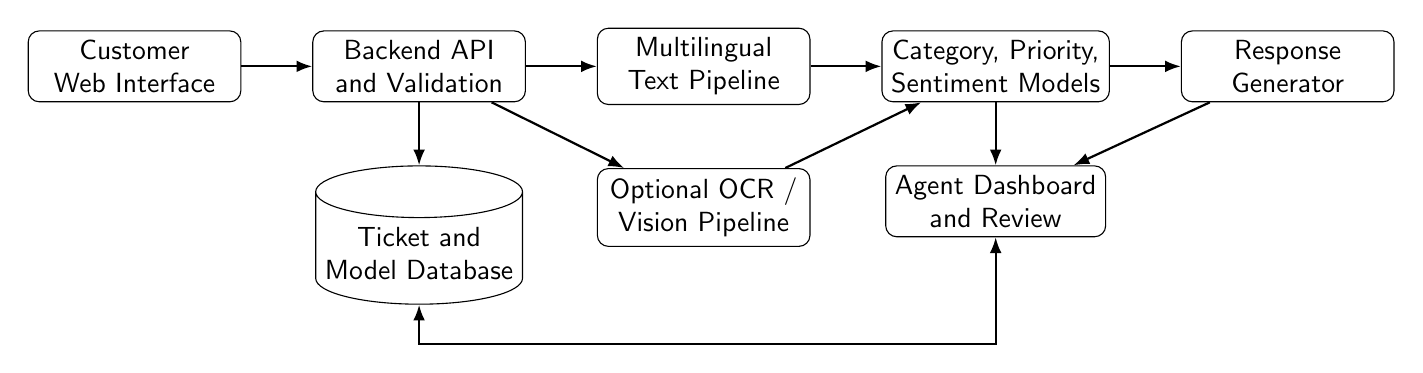
\begin{tikzpicture}[
    node distance=8mm and 9mm,
    box/.style={draw, rounded corners, align=center, minimum height=9mm, minimum width=27mm, fill=white, font=\sffamily\fontsize{10}{12}\selectfont},
    data/.style={draw, cylinder, shape border rotate=90, aspect=0.25, align=center, minimum height=10mm, minimum width=22mm, fill=white, font=\sffamily\fontsize{10}{12}\selectfont},
    flow/.style={-{Latex[length=2mm]}, thick},
    biflow/.style={{Latex[length=2mm]}-{Latex[length=2mm]}, thick}
]
\node[box] (customer) {Customer\\Web Interface};
\node[box, right=of customer] (api) {Backend API\\and Validation};
\node[box, right=of api] (text) {Multilingual\\Text Pipeline};
\node[box, below=of text] (image) {Optional OCR /\\Vision Pipeline};
\node[box, right=of text] (models) {Category, Priority,\\Sentiment Models};
\node[box, right=of models] (llm) {Response\\Generator};
\node[box, below=of models] (agent) {Agent Dashboard\\and Review};
\node[data, below=of api] (db) {Ticket and\\Model Database};

\draw[flow] (customer) -- (api);
\draw[flow] (api) -- (text);
\draw[flow] (api) -- (image);
\draw[flow] (text) -- (models);
\draw[flow] (image) -- (models);
\draw[flow] (models) -- (llm);
\draw[flow] (models) -- (agent);
\draw[flow] (llm) -- (agent);
\draw[flow] (api) -- (db);
\draw[biflow] (db.south) -- ++(0,-5mm) -| (agent.south);
\end{tikzpicture}}
\caption{Main user and software interfaces of the prototype.}
\label{fig:interface-flow}
\end{figure}

\subsubsection{Hardware Interfaces}
Users shall enter text through a keyboard or touchscreen and may upload images from a camera or storage device. No specialised customer hardware is required. A client device should have at least 4 GB RAM and a modern browser. The server shall have sufficient disk space for the configured datasets, models, tickets, logs, and optional attachments. GPU resources may be used for training but shall not be mandatory for basic demonstration inference unless documented.

\subsubsection{Software Interfaces}
The web client shall communicate with a backend REST API. The backend shall interface with the ticket database, multilingual inference services, optional OCR/vision service, and response-generation component. Interfaces shall use documented request/response schemas and include validation status, model version, processing state, and meaningful errors. Production banking-core integration is outside the first-release scope.

\subsubsection{Communications Interfaces}
Client-server and service-to-service communication shall use HTTPS when deployed over a network. Structured requests and responses shall use UTF-8 JSON unless otherwise documented. Requests shall use timeouts, controlled retries where safe, and error handling so that failure of an optional component does not lose the submitted ticket.

\subsection{Database Requirements}
The database shall store tickets, original and processed text, optional attachment metadata, predictions, confidence values, model versions, response drafts, final responses, assignments, statuses, corrections, evaluation results, and audit events. Dataset records shall retain source ID, language form, translation/transliteration lineage, label, and split. The database shall enforce unique ticket identifiers, required relationships, authorised access, and consistent timestamp storage. Binary files may be stored in object storage with protected references in the database.

\subsection{Licensing, Legal, Copyright, and Other Notices}
The project shall comply with the licences and attribution requirements of Banking77, pretrained models, libraries, OCR/vision components, and LLM services. Personal or financial information shall be minimised, access-controlled, and excluded from public datasets or reports. Research and training data shall be de-identified where practicable. The system shall display that generated responses are drafts and shall not imply that the prototype is an authorised production banking service.

\subsection{Applicable Standards}
The requirements document should follow the supplied institutional SRS template and the principles of IEEE 830-1998. Implementation should follow applicable secure-coding, privacy, accessibility, UTF-8 internationalisation, REST API, and version-control practices adopted by the project team. References to websites shall include an access date, and research claims shall use IEEE-style citations.

% =========================================================
\section{Supporting Information}

\subsection*{Data and Model Evaluation Rules}
\begin{itemize}
    \item Category experiments shall use a held-out test set and report accuracy, macro precision, macro recall, macro F1-score, class-wise results, and confusion matrices.
    \item English performance shall be compared with Sinhala, Tamil, Singlish, and Tanglish performance using the same source-record split lineage.
    \item Translation quality and intent-label preservation shall be checked through a documented validation sample.
    \item Naturally written code-mixed data, when available, shall be evaluated separately from translated or synthetically mixed data.
    \item Priority and sentiment datasets, labels, baselines, metrics, and acceptance thresholds shall be documented independently of Banking77.
    \item LLM drafts shall be evaluated for relevance, language appropriateness, factual grounding, safety, and agent usefulness.
\end{itemize}

\subsection*{Business Rules}
\begin{enumerate}
    \item Only an authorised agent may approve a final response or mark a ticket resolved.
    \item Critical tickets and low-confidence predictions require explicit agent review.
    \item Model corrections become candidate feedback and shall not automatically become approved training data.
    \item Category, priority, sentiment, and generated text shall be presented as model outputs rather than guaranteed facts.
    \item Model, threshold, or label-mapping changes require an authorised user and a recorded version.
\end{enumerate}

\subsection*{To Be Determined}
\begin{enumerate}
    \item Final university, department, member names, and submission/approval date.
    \item Whether all 77 Banking77 categories or an approved subset will be used.
    \item Final multilingual encoder and preprocessing/transliteration approach.
    \item Source and annotation procedure for urgency and sentiment labels.
    \item Final OCR/vision and LLM response-generation components.
    \item Confidence thresholds and quantitative acceptance targets for each task.
    \item Maximum image size, retention period, and deployment hardware.
    \item Availability and size of naturally written code-mixed evaluation data.
\end{enumerate}


\end{templatebody}
\end{document}
